\chapitre{Le sort frappe, le mercredi 20 juillet 2033}{Accoté sur le devant de sa Subaru hybride, }{ Sébastien Larose, le dernier syndiqué de la fonction publique du Québec, observe avec délectation la petite foule qui manifeste devant l’entrée principale du CRG-BSL. La chaude brise matinale aidant, une trentaine de personnes, la plupart de jeunes sexagénaires encore productifs, psalmodient des slogans et brandissent des pancartes. Sur certaines, on a reproduit une image éloquente de Robert Gagnon, alias Dart Vader, empruntée au bulletin de nouvelles d’hier. Sur d’autres, on peut lire sur deux lignes «MONSANTO (biffé d’un X rouge)» et «MA SANTÉ!». Autour d’eux, une dizaine de journalistes ravis de cette aubaine médiatique captent tout ce qu’ils peuvent.}

- Non-non-non au manger mou ! scande-t-on par ici.

- Turco-otte, Turco-otte, Turco-otte, «mange d’la marde» répondit l’écho, chantonne-t-on par là.

Le bonhomme grimace un sourire, ce qui déforme légèrement son bouc plus sel que poivre. Pour la circonstance, il a choisi de revêtir son T-Shirt de la CSN, la grande centrale syndicale à laquelle il a adhéré l’an dernier. Comme il était le seul membre du Syndicat de la fonction publique du Québec, il n’avait eu aucune difficulté à organiser la manoeuvre. Surtout qu’il amenait en dote, un compte en banque appréciable.

\begin{floatingfigure}[l]{40mm}
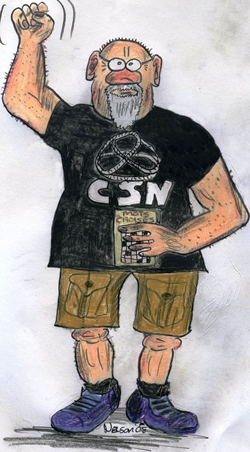
\includegraphics[height=60mm]{corps/chapitre7/img/personnage-sebastien.jpg}
\end{floatingfigure}

- On se croirait revenu à la belle époque. Salut mon homme, fait-il à Timothée qui vient de garer sa voiture à côté de la sienne.

Ainsi Dart Vader est devenu un symbole de lutte ! Pour Timothée, cela ne peut signifier que des ennuis, de très gros ennuis. Ce salaud de Dauphin, l’exécuteur des basses œuvres de Carl Michaud, le directeur général de l’établissement, va sûrement lui faire coiffer la responsabilité, donc la culpabilité, de cette atteinte à l’image de marque du Centre. Mais il se garde bien d’en glisser mot à Larose et file vers l’entrée latérale, celle qui donne directement sur le stationnement. Marie-Odile «la Bitch» Tremblay l’a précédé de quelques secondes devant l’ascenseur et la seconde et quart que durera la montée jusqu’au deuxième leur paraîtra, à tous deux, un siècle et demi. De toute évidence, évalue Timothée, l’agente de sécurité se retient pour ne pas parler d’holotar. Mais pour l’instant, Roméo Du Bellay dort à octets fermés; l’air de ce petit matin sent le concentré de mauvaises nouvelles.

À peine son dispositif personnel polyvalent (DPP) a-t-il avisé le système central de sa présence dans l’immeuble, qu’il se met à vibrer.

- Timothée Tardif !

- Ton chien est mort le Motté !

C’est Flipper Dauphin.

- De quossé ?

- Tu le vois le bordel qu’a créé ton bénéficiaire, ton bonhomme Gagnon ? Ben je vais te le faire récurer, mon salaud. J’m’en vais justement dans le bureau de Carl !

- J’ai rien à voir dans cette histoire, moi ! C’est toi et tes Papyblues qui avez mal fait votre travail…

Mais l’autre a coupé.

- Bof !

Qu’a fait de si terrible Robert «Bob» «Dart Vader» Gagnon, à part se plaindre du manger mou, de dire que ça lui donnait des coliques et de déclarer qu’on le punissait quand il se faisait prendre avec de la nourriture de contrebande ? Quoique à bien y penser…

Arrivé au cinquième, le CS-1 roule sa Saguewanish jusqu’au salon communautaire où une dizaine de vieillards se sont massés devant les fenêtres; la manifestation semble les intéresser.

Le père Jean ne peut se retenir :

- T’as vu, chef, y a encore du monde qui s’rappelle de nous autres !

Timothée laisse border. De toute façon, il n’y a pas plus de Dart Vader dans ce salon qu’il n’y a d’espoir pour une vie meilleure. Vivement, il repart vers le petit dortoir, une salle 2P, où il croit pouvoir le trouver. Pourtant, là non plus, pas d’homme à la canule.

- Il est parti en bas saluer son public, fait le vieux Martel.

- Où en bas, monsieur Martel ?

- En bas.

- Shit !

- Le prophète Abdias a dit : «Comme tu as fait il te sera fait : tes actes te retomberont sur la tête.»

- Ta gueule, Savoie, gronde Martel, tu nous écœures !

Mais Timothée est déjà en route vers le rez-de-chaussée. Sur place, il remarque son ami Shimoune Saint-Pierre, dit la grande folle du manger mou, en train d’écornifler. Partout, des agents de sécurité montent la garde et, près de l’accès à la cafétéria, un des sbires de Philippe Dauphin, soit Bluesly, soit Papynut, en tout cas, un des frères Côté, fait les cent pas, concentré sur sa boucle d’oreille. À ce qu’il semble, la plupart des pensionnaires ont choisi de se faire rares.

- Ils l’ont amené, annonce Saint-Pierre.

- Qui a amené qui, Shimoune ?

- Les Papyblues. Ils viennent de partir avec Dart Vader.

Saint-Pierre a imité le geste du bonhomme quand il appuie sur sa valve de phonation.

- Pour où ?

- Devine !

Et Shimoune de repartir vers son centre nutritionnel.

S’il n’était pas si «timoroso», Timothée foncerait sur-le-champ protester à la direction générale. Des gorilles ont escorté son pensionnaire vers l’inconfort du sous-sol où il sera puni pendant deux semaines ? Un mois ? Plus ? Cela, pour avoir dit publiquement ce qu’il pensait, pour avoir dit la vérité. Mais une esquive le sauve de sa couardise; son lobe d’oreille se met à frétiller.

- Timothé Tardif !

- Motté, c’est Laurent !

Encore des ennuis, soupire le CS-1.

- Alors ?

- Le père Lafrance vient de se lâcher, p’is ça pue la charogne. Y a plein de bénéficiaires qui chialent. Y a du vomi sur le plancher, sur la commode, sur les pattes du lit.

- Bon, je monte.

Arrivé au cinquième, il remarque, en croisant le salon communautaire, que la pièce a fait son plein de vieillards. Tout le monde est là et tout le monde a son idée sur la manif. Le pire, c’est qu’à l’exception de Jean Saint-Gelais, cet indécrottable délinquant, ils seront probablement tous ravis quand ils apprendront pour Dart Vader. Mais on n’y peut rien; c’est ainsi; le bonhomme l’a sans doute cherché.

Sauf que pour l’instant, il y a une urgence désagréable à gérer et ce ne sont ni Laurent, ni Mérovée, ni lui, qui nettoieront l’horrible dégât. Quant à faire venir une équipe du service d’entretien, c’est impensable. Il faudra patienter une bonne journée avant qu’elle ne se pointe. Il serait surtout important d’avoir une petite caisse garnie pour pouvoir bien arroser leur coordonnateur.

Cette annonce lui fait penser à la puanteur remarquée l’autre jour dans une des deux salles 2P-F, celles qui sont réservées aux femmes. Et puisque tout le monde semble être au salon, pourquoi ne pas en profiter, en chemin, pour aller redonner un coup de nez dans ce triste local, question d’en avoir le cœur net ? Bonne idée ! Mais en y entrant, le CS-1 tombe sur une scène romantique, mais pas encore torride, où, avec force soupirs, madame Thériault essaie de faire des choses discutables à madame Labbé dans le lit de cette dernière. Dieu du ciel !

- Que c’est que je vous ai dit avant-hier, madame Thériault ?

La rondelette créature se glisse en bas du lit et, en souriant à sa conquête, s’en va s’asseoir sur le sien.

- On faisait rien de mal, hein Jeanne ?

- B’en non, ment l’autre, une maigrelette aux allures d’alitée permanente.

Normalement, Timothée aurait baissé la tête et serait ressorti aux commandes de son bruyant Saguewanish. Mais pas cette fois. L’occasion est inespérée.

- Madame Thériault, si je veux, je n’ai qu’à descendre au 2e, aller à la Sécurité, leur demander un disque de la dernière heure ici dans cette salle 2P, amener ça au premier, chez les patrons, et, dix minutes plus tard, deux gros Papyblues qui haïssent les gouines, vont venir vous chercher, vous et madame Labbé, et ils vont vous descendre au sous-sol avec les autres foqués.

Il est venu près de dire «avec Dart Vader».

Les deux coquines déglutissent. C’est madame Thériault qui réagit, estimant probablement, en son for intérieur, qu’elle est la plus coupable des deux.

- Si tu veux ?

- Si je veux.

- C’est quoi le «si» ?

Timothée prend une grande respiration et il médite, une ou deux secondes, sur l’image de sa mère. Celle qu’elle avait avant sa réclusion dans un sous-sol de Nazareth. Celle qu’elle affichait quand elle lui enseignait si méchamment le trombone.

- C’est un plancher de vomi à nettoyer !

Grimaçante, madame Thériault est assez ratoureuse pour ne pas se mettre à hurler. Elle veut plus de détail.

- Le pére Lafrance, ici à côté dans la salle 3P-L, il a rendu tout ce qu’il avait dans le corps. Je vais devoir le transférer en palliatif. Pas drôle. Y a du vomi sur le plancher, sur la commode, sur les pattes du lit. C’est écœurant.

La bonne femme réfléchit un instant.

- J’peux-t-y avoir de l’aide ou faut que j’soye toute seule ?

- J’te vois v’nir, ma snoroune, s’insurge immédiatement l’autre coquine. C’est pas moi la turbo lesbo, c’est toi !

Timothée chasse une pensée fugace sur la mesquinerie de ses frères et sœurs humains.

- Celles qui torchent propre propre ne vont pas chez les foqués. Celles qui restent sur leur cul y descendent pour longtemps longtemps.

Une minute plus tard, le trio entre dans le dortoir des cas lourds en ce qui a trait à la perte d’autonomie. Une odeur épouvantable, soutenue de gémissantes protestations en provenance des lits, les accueille. Robespierre, en voisin de bureau, s’est arrêté près de la porte et tente de respirer le moins possible.

- Je peux te donner un coup de main ?

- Non, merci, t’es gentil. Mais j’ai ce qu’il faut.

Il pointe vers les deux délinquantes.

- Monsieur Lafrance, on s’en vient vous aider, annonce Timothée au grabataire souillé. C’est madame Thériault avec madame Labbé – vous les connaissez, non ? – qui vont vous ramasser ça. Quand elles ont appris votre malheur, elles se sont dépêchées.

Le bonhomme fixe le CS-1 de ses grands yeux noirs.

- J’veux pas m’en aller dans la salle palliative ! J’suis encore bon ! J’suis pas fini !

Timothée fait mine de rien et se retourne vers les deux femmes.

- Les moppes, les guenilles, le savon sont dans le placard 5-PP67, juste à côté dans le couloir. Je vous l’ouvre.

Il appuie alors sur son sa boucle d’oreille et déclame :

- Ouverture ! CS-1 Timothée Tardif ! 5-PP67 ! Oui !

Ce qu.entendant, les commères vont quérir leur matériel. Rassuré, le fonctionnaire manœuvre son Saguewanish vers la porte en contournant l’immonde flaque du père Lafrance. Mais celui-ci veille au grain et il tend la main.

- Attends une minute, mon ‘tit Motté, j’ai un cadeau pour toé !

- Un cadeau ?

- Pour rester ici, pour pas aller chez les morts. J’ai ramassé 642 piastres.

Mais il n’a pas de bout de papier avec un code inscrit par Solange Gadoury. Le CS-1 commence par vouloir décliner, par vouloir lui crier que c’est trop, que la situation est horrible, par vouloir lui jurer qu’il refuse de lui voler ses dernières économies, qu’il en aura besoin quand il sera en SP en train d’attendre la prochaine cérémonie de groupe. Mais, encore une fois, l’image de sa mère vient se substituer. Quelle tempête elle fera si elle apprend qu’il a refusé 642 \$ ! Ainsi, Timothée accepte en fuyant le regard du moribond. Pour la Maririou, pour Romain, il prendra cette somme, pour peu que la mère Gadoury lui en donne le code.

Auquel cas, par la volonté d’un fonctionnaire qu’il vient de graisser, Jean Lafrance ne sera pas conduit dans l’antichambre de la mort du 5e Nord. Du moins pas pour l’instant.

Une voix se fait entendre du couloir, celle du bonhomme Saint-Gelais.

- Vous vous êtes faites pogner, les gouines ?

- Étouffe-toi donc, vieux maudit, lui rétorque la mère Thériault.

Tout au fond de son sombre local, le vieux Asselin est assis à la noirceur, dans l’unique fauteuil de la pièce.

- Pas besoin d’avoir des yeux pour savoir qui vient me voir sur sa bécane. Y a seulement la tienne, chef, qui fait tant de bordel.

- Bonjour Monsieur Asselin. Comment ça va aujourd’hui ?

- Juste au son, ton moteur devrait sauter d’ici dix à quinze kilomètres.

Timothée fouille dans le porte-documents accroché à son Saguewanish.

- Branchez-vous ce lecteur à l’oreille. J’y ai mis l’œuvre complète de Tchekhov.

Les lèvres du vieillard tremblent et ses longs doigts se referment sur le gadget chinois.

- Je pèse où pour que ça parte ?

Timothée lui place la main au bon endroit.

- Essayez de dormir quand même.

L’entorse au règlement risque de lui faire chauffer le matricule si les cafards télécommandés du 2e attirent l’attention d’un agent de sécurité (agente de sécurité ?) mal intentionné. Mais il s’en fiche. Il éprouve même une grande satisfaction de l’avoir fait.

Encore une fois, l’oreille lui chatouille. Décidément !

- Timothée Tardif !

C’est la voix de son père.

- Viens-t-en vite. C’est ta mère ! Elle n’arrête pas de saigner.

- Maman ?

- Ça a commencé tantôt.

Du sang, sa mère saigne. Le cœur de Timothée s’est accéléré.

- Elle saigne, comme une hémorragie ?

- Oui. Ça vient d’en dedans. Ça lui sort par le milieu. Je sais plus quoi faire !

Sans aviser quiconque, en évitant de regarder Bea Bellow qui, livres en main, a tenté d’attirer son attention, le fonctionnaire file vers le stationnement et roule, le plus vite qu’il le peut, jusqu’à chez lui.

Plein d’appréhensions, Timothée veut descendre l’escalier. Mais Gazou, le chien-rat, lui bloque l’accès. La sale bête semble enragée au point de vouloir le mordre. Sans hésiter, il l’attrape par la tête et, comme s’il s’agissait d’une peluche que l’on jette aux rebuts, la propulse littéralement à la rue.

- Kaï kaï kaï !

Vive les colliers GPS !

En bas, il trouve son père assis sur le bord du lit où geint une Maririou en état total de panique. Il lui a placé des serviettes, mais, il ne fournit pas. On dirait que la vieillarde est en train de vidanger son méchant. En plus de ne rien comprendre de ce qu’il lui arrive, elle voit bien le dégât causé par ses saignements abondants, ce qui a l’heur de l’angoisser davantage.

- Mon Dieu Cheigneur, qu’est-che qui m’arrive ? Que ch’est que je vas faire ?

Sidéré, Timothée se tait. Il regarde, il essaie de comprendre. Elle saigne ! Elle coule ! Et du vagin ! Sa mère ! Comment pourrait-il arriver à la toucher, à toucher au vagin de sa terrible mère, au terrible vagin de sa mère ? Il a beau connaître les premiers soins, il est impuissant.

- Va vite me chercher d’autres serviettes. Dépêche !

Tandis que le fils accourt jusqu’au placard lingerie, comme s’il voulait fuir le long geignement sans accalmie de sa mère, Romain, lui, ne réfléchit plus. Il éponge le pire. Il maintient une serviette sur la source morbide. Il tente de se faire rassurant.

- C’est moins pire que tantôt, ment-il à sa compagne dont la pâleur commence à être inquiétante. On dirait que ça ce calme.

- J’vas mourir, Romain.

- Tais-toi donc. Ça va s’arrêter. Crois-moi !

Et là, phénomène excessivement rare, la Maririou se met à pleurer d’un sanglotement effrayé, charnel, profond, une longue plainte qu’on dirait associée à la mort, une insoutenable lamentation où on peut décoder quelques « j’vas mourir ». Gauchement, Romain essaie de la réconforter, mais, comme peut le constater le fils, il n’y arrive pas du tout. La panique est même en train de le gagner. On n’a plus le choix; il faut d’urgence aller chercher de l’aide. De l’aide discrète, si possible !

\begin{floatingfigure}[l]{40mm}
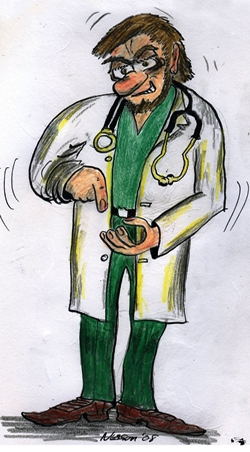
\includegraphics[height=60mm]{corps/chapitre7/img/personnage-etienne.jpg}
\end{floatingfigure}

- Y a Étienne Gagnon, dit-il d’un ton deux coches trop élevées. C’est un des médecins du Centre, un gars qui trempe dans toutes sortes de combines.

- Y est-y capable de soigner ta mère ?

- Il connaît son affaire, mais ça va nous coûter un bras et on n’a même pas 2 000 \$ dans le compte !

- On n’a pas le temps de calculer, va vite le chercher !

Timothée file et, sans un regard pour Gazou qui voudrait bien revenir vers sa maîtresse, fait démarrer son antiquité sur les chapeaux de roues. D’un tic de l’index sur sa boucle d’oreille, il demande à la réception du Centre si le docteur Gagnon est sur place où s’il est à sa clinique privée du quartier Saint-Germain, un secteur assez huppé de Rimouski. La deuxième possibilité serait vraiment géniale, se dit-il.

La chance lui sourit. Non seulement le médecin y est, mais il accepte de le recevoir entre deux rendez-vous.

Devant la gravité de la situation, le toubib met fin abruptement aux négociations.

- Ça sera mon prix ! C’est à prendre ou à laisser. On n’a pas le temps de négocier; ça presse !

Comme son interlocuteur donne un signe d’acquiescement, il demande à sa réceptionniste d’informer tout le monde qu’il a dû partir pour une urgence et d’essayer de tout décaler de deux heures.

- C’est beau, je te suis !

Une heure plus tard, Marie a cessé de saigner et, la bouche édentée grande ouverte, elle dort avec bruyante application. Et pour cause; Gagnon, en émule de vétérinaire, lui a administré un sérieux cocktail pharmaceutique. Il a toutefois fallu que Romain mette Gazou sur la petite galerie face au fleuve, la mauvaise bête s’étant réintroduite dans la maison à l’arrivée des secours, une arrivée hautement remarquée par Louis-Marc Richard, d’ailleurs.

- Elle a quoi ? demande Romain.

- Un beau cas de métrorragie ou, si vous préférez, d’hémorragie postménopausique. C’est clair qu’il y a un problème à l’endomètre. À son âge, ce sont peut-être des polypes endométriaux, des polypes qui sont là de façon latente depuis des années. Sinon, il peut s’agir d’une tumeur. Faut aller voir.

- Une tumeur ? Un cancer ?

- Les tumeurs ne sont pas toujours malignes.

- Faut aller voir comment ?

- Faudrait lui passer une échographie. J’ai ce qu’il faut, un système portatif Bluetooth Azure. Si ce sont des polypes, on verra pas grand-chose. Mais si c’est une tumeur, on verra une masse. Malheureusement, on ne pourra pas savoir si elle est cancéreuse. Pour le savoir, va falloir une analyse sanguine avec une recherche spécifique de marqueurs susceptibles de confirmer ou d’infirmer la présence de cancer. Sauf que ça va coûter des bidous; mon technicien ne vit pas avec l’air du temps !

- Seigneur !

- S’il y a tumeur, cancéreuse ou non, il faut l’enlever. Et là aussi, j’ai ce qu’il faut. Je peux pratiquer ici même une hystéroscopie qui pourra régler le problème. Évidemment, il lui faudra du repos et une médication appropriée, peut-être pas des progestatifs à son âge, mais quelque chose pour éviter l’infection, favoriser la cicatrisation et réduire la douleur.

- Ça a pas de maudit bon sens !

- Il va falloir que je revienne avec mon matériel médical le plus tôt possible, possiblement demain en matinée. En attendant, vous lui faites prendre ces pilules-là et celles-là, trois fois par jour, juste avant de manger.

- Oui mais docteur, balbutie Timothée, on n’est pas capable de payer tout ça !

Gagnon caresse son collier de barbe.

- Je sais. Tu ne roules pas sur l’or et, en bon fils, tu te saignes pour héberger tes parents, deux Boomers illégaux. Si je te demande de l’argent, tu vas péter au frette ! Donc je ne t’en demanderai pas.

Le cœur du «bon fils» veut lui sortir de la cage thoracique.

- Mais …

- … je vais te demander un petit service.

Timothée ravale cette salive fétide qui lui gâche l’haleine.

- Un service ?

- Oui. Il me faut certains produits, des produits pharmaceutiques, parmi ceux qu’ils utilisent au centre nutritionnel pour «assaisonner» les plats de Nutrisuz. Peux-tu m’aider ?

- Des produits pour ma mère ?

- Non. Ça rien à voir. C’est pour ma business. C’est donnant donnant. Je soigne ta mère, tu me procures des produits dont j’ai besoin pour d’autres patients.

Horriblement angoissé, le quadragénaire enlève ses verres et les essuie avec le pan de sa chemise. Dehors, Gazou a cessé de japper et a commencé à hurler.

- Il va nous attirer les voisins ! Déjà que tantôt, Louis-Marc Richard nous a vu arriver, le docteur et moi !

Romain lui ouvre la porte et, du pied, l’oblige à demeurer dans la chambre de sa maîtresse. Sauf que Gazou est déchaîné.

- Tais-toi, asti de chien fifi ! J’vais te fesser à coups de soulier !

Comme s’il avait compris, le chien jaune s’en va renifler près du lit de la vieillarde et, prouesse étonnante compte tenu de son embonpoint et de la longueur de ses pattes, saute sur l’édredon recouvrant la malade.

- Je veux bien vous aider, docteur, mais je n’ai pas accès aux produits pharmaceutiques du Centre, moi. Le seul qui puisse pigrasser là-dedans c’est Amédée Chicot. À part lui, je vois pas qui peut vous aider. Mais ça, vous devez bien le savoir ?

Tandis qu’il referme soigneusement sa petite mallette de toubib comme il y en avait dans les anciens films, il lève les yeux en direction de Timothée.

- Je vais te dire comment je vois ça. Tes parents, ta mère surtout, ont un urgent besoin de soins professionnels et mon serment d’Hippocrate m’oblige à m’assurer qu’ils en aient. Or voilà que je peux leur en fournir, mais c’est ainsi que ça fonctionne, il y a des frais, des frais que tu dois assumer. Si tu n’es pas capable, mon devoir est de m’assurer que tes vieux parents reçoivent quand même des soins. Et dans le domaine du gratuit, je ne vois pas d’autre solution que celle du CRG.

- Oui, mais mes parents sont illégaux …

- C’est pas mon problème. Leur santé, que dis-je, leur vie passe avant tout.

- Je sais, mais …

- Écoute, je ne te demande pas le Pérou. Y vraiment rien d’extraordinaire là-dedans. Depuis que c’est Michaud qui est DG au Centre, tout le monde se sert; le vol est devenu pandémique. Prends le temps d’y penser, d’imaginer une solution et fais-moi signe quand tu auras trouvé … disons d’ici une semaine ?

Sur cette tirade, le bon docteur gagne la sortie.

Complètement défait, accablé, découragé, Timothée arrive quand même à voir le salopard disparaître dans l’escalier, accompagné du chien-rat hurlant de toute sa haine. Une lueur assassine aux yeux, le toubib tente, d’un rapide coup de pied, de le faire retraiter, mais Gazou esquive le danger et poursuit son insupportable manège. Encore une fois, Romain doit s’en mêler.

- Gazou, ciboire de bâtard de chien débile, ici, au pied !

Subodorant les conséquences d’avoir fait lever le bonhomme, l’horrible roquet retourne se réfugier en grondant auprès de sa maîtresse.

- Serment d’Hippocrate, serment d’Hippocrate ! Sacrament d’hypocrite de maudit hypocrite de sacrament !, sanglote nerveusement Timothée sans regarder son père.

Comment il va faire pour dénicher les produits que convoite Étienne Gagnon ? Tout est tellement surveillé dans l’établissement ! Quand bien même qu’il en parlerait à son ami Shimoune, ça ne donnerait pas grand-chose. Tout au plus connaîtrait-il les heures où il est possible de passer au centre nutritionnel sans qu’il n’y ait de préposés. Mais encore là, sans code pour déverrouiller la remise pharmaceutique, comment pourrait-il aller plus loin ? Arriver avec une hache de sapeur camouflée dans sa chemise ? Avec une pince monseigneur ? Soyons réalistes! Et la pire difficulté n’est même pas à ce niveau. Elle est au 2e, chez les gens de la Sécurité qui, avec leur électronique de pointe, voient tout et entendent tout à la grandeur du bâtiment. Pire, des détecteurs savent déceler les articles qu’apportent, cachés ou non, les employés qui entrent dans l’établissement ou qui le quittent.

Soudain, un flash lui permet d’extirper d’un recoin perdu de sa mémoire le nom de cet ouvrage d’Orwell qui lui avait traversé l’esprit l’autre jour : 1984 !

L’inquiétude lui rongeant le système, Timothée regarde sa montre; il n’est pas encore 13 heures. Il doit absolument retourner au Centre pour régler quelques trucs; il ne faut quand même pas attirer l’attention. Vérification faite dans sa boucle d’oreille, il sait qu’aucun message de Carl Michaud ou de Flipper Dauphin ne lui est parvenu. Bonne nouvelle ? Pas certain ! Demain c’est la réunion du Comité de déontologie dont il fait partie et où siègent ces deux hauts gradés. Il est probable qu’ils en profiteront alors pour lui faire sentir leur courroux.

- Je reviens dans une heure, fait-il à son père qui, malgré l’hostilité de Gazou, est retourné s’asseoir sur le bord du lit de sa vieille compagne.

Comment ne pas penser à cette énorme tuile qui vient de lui fracasser son misérable ordinaire ? Comme faire semblant qu’il n’y a aucun problème à part sa trottinette qui est en train d’agoniser bruyamment ? Dans sa salle palliative où il se rend tout d’abord pour bricoler de la paperasse en vue de la Cérémonie de groupe du 3 août prochain, une vieille dame, l’occupante du lit no 5, lui fait un signe discret. Quand il se penche sur sa couchette, elle lui dit qu’elle ne veut absolument pas «assister» à la «prochaine célébration» et qu’elle a un petit accommodement à lui proposer.

Outre l’aspect extraordinaire du fait qu’il s’agisse de la deuxième tentative de pot-de-vin de la journée, ce qui rend ce cas vraiment touchant, c’est que la mère Gadoury n’a pu lui dénicher que 200 \$. À ce tarif, on s’en doute bien, personne du CRG-BSL n’accepterait de trafiquer un dossier de bénéficiaire. Mais Timothée, lui, il y consent. Le regard de la mourante est tel, qu’elle ne lui aurait offert que dix sous et il aurait dit oui. Le 3 août, c’est dans quinze jours et, pense-t-il, la pauvre dame, dans l’état où elle est, ne vivra sûrement pas jusque-là. Le calcul est simple : si ce n’est pas lui qui empoche les 200 \$, ce sera le Centre, c’est-à-dire le gouvernement. Cet État on ne peut plus vorace. Aussi bien que l’argent serve à ceux qui en ont vraiment besoin. De toute façon, eux, ces vieux qui casquent à coups de petits 200 \$, ils se paient de l’espoir sur leur grabat de mourant. Et ça, c’est bien. Oui mais le mythique Timothée de Milet n’aurait sûrement pas, lui, accepté de fric, lui, et aurait vidé l’établissement de tous ses profiteurs à grands coups de lyre à onze cordes. Mais, bof !

Dans son bureau, il aimerait pouvoir vérifier et modifier la fiche de cette mourante, ne serait-ce que pour s’occuper les méninges, pour donner aux autres l’impression que tout est comme d’habitude, que sa mère ne vient pas de chambouler inexorablement le scénario de leurs trois vies. Mais, encore une fois, rien ne fonctionne du côté informatique centrale. Ne reste plus qu’à tout fermer et rentrer à la maison ! Comme s’il pouvait y avoir présentement un ailleurs !

Rue Crouet, il retrouve son père assis devant une télé sans audio, perdu dans ses pensées. Le vieillard le salue vaguement de la main. Gazou n’a pas jappé. Couché sur le bout du lit où ronfle la Maririou, il s’est contenté de gronder.

- Tire-toi une bûche.

Mais Timothée sait que la conversation sera difficile. Romain est amer. Ce qui devait arriver s’est produit. Sa Marie est tombée gravement malade. Plus rien ne va et demain sera encore plus épouvantable qu’aujourd’hui. Il ne peut en être autrement. Si ce n’est ce «crosseur de médecin» qui va les dénoncer, ce sera le voisin d’en face, cet «enfant de chienne» de Richard qui le fera ! Est-ce la fin du parcours ? Est-ce un aller simple vers les geôles du CRG ? De toute façon, avec cette maladie, il doit être devenu trop tard, maintenant, pour vraiment considérer la fuite vers Anticosti.

- Oui, mais j’ai pas eu le choix, fallait que je me grouille ! Et mis à part le docteur Gagnon, je ne voyais personne d’autre !

- Je sais. Tu as fait de ton mieux. C’est pas après toi que j’en ai, mais après le sort !

Timothée ravale un sanglot.

- Ta mère avec son caractère de chien, avec ses exigences jamais satisfaites, elle t’a toujours beaucoup aimé.

Et le bonhomme que l’on dirait claquemuré dans ses souvenirs se lance dans l’exposé sans fioritures, d’un pan de vie que Timothée aurait tellement souhaité pouvoir oublier. Un pan qui aura duré presque dix ans et dont les protagonistes étaient sa mère et lui. Résigné, il réentend l’histoire de cette matrone sans pitié qui, soir après soir, lui faisait refaire ses devoirs, reprendre ses études, récapituler ses leçons. Encore une fois, son père lui raconte la persévérance de cette femme autoritaire qui, année après année, tenait tête aux enseignants, aux spécialistes, aux directeurs d’école qui voulaient de concert recaler son cancre de fils, l’affecter aux classes spéciales ou le changer d’institution. Il laisse Romain lui remémorer le calvaire de cette Maririou avare de sourire et dépourvue d’affection, qui l’avait amené à réussir, bien malgré lui, son primaire, son secondaire et, en partie, son collégial. Dieu qu’elle lui en avait fait baver !

- Mais, elle a jamais pu dire «je t’aime» à personne. Ni à moi, ni à toi !

Dans sa chambrette voisine, la Maririou s’est mise à balbutier d’incompréhensibles arguties.

Le fils enlève ses verres et, des paumes, se frotte les yeux brûlés d’émotion. Que peut-il faire ? Est-ce la fin de ses parents ? Deviendront-ils les prochaines proies des flics du BAG ? Et lui ? Qu’arrivera-t-il de sa carrière une fois que toute l’histoire aura été révélée ? C’est jeune, 43 ans, pour vivre dans la dèche, pour faire de menus travaux afin de pouvoir manger et être soigné, pour aller changer des couches de vieux sous les quolibets de tout le monde, y compris des incontinents eux-mêmes. Existe-t-il une solution ? Est-ce possible de la découvrir d’ici une semaine ? C’est court une semaine ! Le temps est-il venu d’utiliser les pilules de Robespierre ? Faudrait-il commencer à en parler à Romain ?

La peur et l’angoisse le font plutôt filer. D’une traite, il se rend jusqu’au cimetière tout près de sa maison. Lentement, il s’appuie sur la clôture, comme pour mieux goûter l’air parfumé de cette superbe journée de juillet, un air venu tes terres plus au sud, un air très doux où les effluves d’avoine fraîche laissent passer celles, plus sucrées, du trèfle rouge. Derrière lui, plus loin, à sa droite et à sa gauche, des éclats de joie, de plaisir sportif, de jeux d’adultes lui parviennent. Nazareth semble d’humeur joyeuse. Il fait beau, les gens sont heureux. Même les morts du cimetière doivent l’être. Le seul qui ne l’est pas c’est lui, ce bon fils d’une mère très malade dont la vie, jusque-là pas si extraordinaire, est en train de basculer, par son sang, vers le pire des cauchemars.

Méchante journée !